\setcounter{chapter}{1}


\chapter{Related Work}
\label{ch:related-work}



Information foraging~\cite{Pirolli1999}, or the process through which an individual 
obtains knowledge that assists them accomplish a task often experiences paradigm shifts. 
At times, 
an information need was directed to a library clerk 
who would direct an individual towards 
sections of the library with books pertinent to the question 
posed by a person~\cite{saracevic1975}.
Then, when the \acf{web}~\cite{berners1994web} became popular,
individuals started to rely on search engines 
to seek information~\cite{Page1999} now digitally stored in the form of web pages.
Searching for pertinent artifacts, be them books or web pages, 
is one of the first steps to address an information need,
which we detail in Section~\ref{cp2:searching}.


Then, in possession of a pertinent artifact, careful 
inspection of its content might lead a person 
to find the information that they sought. 
However, due to some of the challenges
associated with finding pertinent information within 
an artifact discussed in the previous chapter, researchers from several 
disciplines have considered means to help 
in this activity. 
In Section~\ref{cp2:general-approaches}, 
we detail approaches from related work
that have investigated how to automatically identify relevant text. 
Then, in Section~\ref{cp2:task-approaches}, 
we hone in approaches 
for automating the identification of text 
likely relevant to a software task.




% Most of the techniques that extract information from natural language software artifacts
% are examples of applications that help developers in performing 
% software development activities~\cite{Meyer2017}. 
Given how 
natural language artifacts have become intrinsically
tied to software development~\cite{umarji2008archetypal},
we conclude this chapter with an overview of 
other applications that make use of textual data
to help developers
across many of the tasks in their daily work (Section~\ref{cp2:dev-productivity}).
\art{v4.0}


% In the last chapter, we introduced some of the challenges
% associated with finding
% information relevant to a developer's task.
% In this chapter, we provide background information on 
% a number of empirical studies that give insight into
% the data available in natural language software artifacts 
% and we also present 
% automated tools that extract text from these artifacts.
% In Section~\ref{cp2:text-in-se}, we begin by providing an  
% overview of the types of textual analysis in the literature
% then, in Sections~\ref{cp2:general-approaches}
% and~\ref{cp2:task-approaches}, we
% detail general textual approaches 
% and task-specific approaches
% that identify and extract text from natural language software artifacts, respectively.
% First, we provide an overview on the kinds of approaches 
% used to extract data from natural language software artifacts.
% Then, we detail how these approaches 
% have been used for automating the identification of text 
% likely relevant to a software task~\cite{a}.







\section{Finding Pertinent Artifacts}
\label{cp2:searching}


We start by considering how an individual finds 
artifacts, or documents, which might 
address an information need. 
For this, information foraging theory~\cite{Pirolli1999} explains how a person navigates through  
a search space looking for information patches  based on 
a set of cues about the effort and gains that a patch provides to them~\cite{Pirolli1999}.
A patch can represent both search results or the content within an artifact
and \textit{explicit} or \textit{implicit} factors affect judging the relevance 
of an information patch~\cite{saracevic1975}.
For example,
consider an electronic library catalog and a search for `\textit{android notifications}'.
Figure~\ref{fig:library-catalogue} shows two hypothetical results for this search
to help ilustrate explicit and implicit factors.
An explicit factor might represent how the keywords in the `\textit{subject and genre}' 
directly match one of the keywords used in the query. An implicit factor might represent 
a person's background or previous knowledge, such as how 
the person performing this search 
might know that the first book targets a more general population and 
that it might not be helpful for a software developer.





\vspace{3mm}
\begin{figure}[H]
\noindent\fbox{%
\parbox{\textwidth}{%
{\ttfamily% 
    \begin{scriptsize}
        \begin{enumerate}[itemindent=-1em,leftmargin=1em]
            \item \textbf{Android for Dummies} 

            Author: Gookin, Dan 

            Location: Britannia Branch Library 

            LC Call No.: 004.167 A57G6ad 

            Subject and genre: Android (electronic resource), Smartphone, Mobile computing

            % Synopsis: This book will tell you pretty much everything you need to know about your Android smartphone or tablet in an equally friendly manner, because that's the best way to learn how to get the most from your Android

        \end{enumerate}          
    \end{scriptsize}
    }%
}}
\noindent\fbox{%
\parbox{\textwidth}{%
{\ttfamily% 
    \begin{scriptsize}
        \begin{enumerate}[itemindent=-1em,leftmargin=1em]\setcounter{enumi}{1}
            \item \textbf{Learning Android} 

            Author: Gargenta, Marko 

            Location: Champlain Heights Branch Library 

            LC Call No.: 005.44 A5G2L1 

            Subject and genre: Android (electronic resource), Application software (development), Mobile computing

            % Synopsis: Presents an introduction on the fundamentals of Android to create a variety of applications.

        \end{enumerate}
    \end{scriptsize}
    }%
}}
\caption{Sample library catalog with two results associated with the keyword `android' }
\label{fig:library-catalogue}
\end{figure}




A similar search could be performed on a web search engine\footnote{e.g., \href{https://www.google.com/}{Google} or \href{https://www.bing.com/}{Microsoft Bing}}
and for both library catalogs or web searches, researchers have investigated 
what affects how a person finds pertinent results and their decision to inspect them.
For example, in electronic library catalogs,
Hildreth observed how keyword searches were used more than any other type of searches (e.g., by author or by title)~\cite{hildreth1997}
while other 
others studies observed impatience and near-random search habits in novice librarians~\cite{novotny2004don}.
In contemporary web search engines, researchers have  also 
investigated how individuals formulate queries~\cite{gross2005have, bendersky2012},
how prior knowledge helps them
to more efficiently perform searches~\cite{DeGraaf2014},
and what search results they inspect, going to the lengths
of using eye-tracking technology for this purpose~\cite{Cutrell2007, marcos2015}.



With the prominence of web search engines, other search problems also gained attention.
For example,  Carbonell and Goldstein pioneered the need 
to investigate both the relevance and novelty of search results~\cite{Carbonell1998}.
That is, on one hand, if one returns only relevant resources, it may be the case that all results contain redundant information 
which might leave some information needs unanswered. 
On the other hand, if the search results are too diverse, it might be difficult for an individual 
to find information that corroborates and consolidates some conclusion~\cite{clark2013relevance}.  
This has led researchers to investigated 
how to balance the relevance and novelty of the results retrieved
by a web search~\cite{najork2001, rafiei2010, vieira2011}
and commercial search engines have since considered how to strike a balance
between relevance and novelty.





Across these general studies, and also in software engineering-specific studies~\cite{Starke2009, Brandt2009a, DeGraaf2014},
a common trend is that the identification of good search terms is as, or even more
important than the search algorithm itself~\cite{Kevic2014}. 
Nonetheless, identifying good search terms is often challenging~\cite{novotny2004don, Haiduc2013} and 
as a consequence, many searches are unsuccessful or retrieve resources that 
a person loses time inspecting only to find that they are not pertinent to the task at hand.
This indicates that individuals usually inspect multiple types of artifacts 
before finding relevant information, further motivating
the work presented in this thesis.



% which contrasted how more experienced users were able to better translate an information 
% need into keyword searches that retrieved useful results



% \section{Automatic Approaches for Identifying Text in Natural Language Software Artifacts}
\label{cp2:text-approaches}



Information useful to a software task can be buried in irrelevant text or attached to 
non-intuitive blocks of text, making it difficult to discover~\cite{Robillard2015}.
Researchers have long recognized the value of assisting developers in 
identifying information of relevance in this natural language
text.
In this section, we detail tools and approaches from related work.




\subsection{Pattern Matching Approaches}
\label{cp2:pattern-matching}


Pattern matching approaches rely on regular expressions describing a sequence of tokens that represent
 a relevant text fragment~\cite{Bavota2016}. Tokens can either represent words or linguistic elements 
extracted using \acf{NLP}.
    
    
As examples  of pattern matching approaches,  {\small DeMIBuD}~\cite{Chaparro2017}
 and Knowledge Recommender (Krec)~\cite{Maalej2013, Robillard2015} are tools that detect relevant sentences in bug reports and API documentation, respectively. 
These tools derive a set of patterns from annotated data and use them as part of heuristics 
that identify relevant text. Krec assumes that any relevant sentence mentions a 
code element (e.g., a class or method name) and it uses  361 unique patterns
to 
detect relevant sentences in API documentation~\cite{Robillard2015}.
In a similar manner, {\small DeMIBuD} uses a set of 154 discourse patterns to detect sentences 
relevant to understanding a bugs observed or expected behaviour and steps to reproduce it,
which are essential to bug triaging tasks.




In Stack Overflow posts,
Nadi and Treude~\cite{nadi2020} have both applied the original set of patterns from Krec~\cite{Robillard2015} 
and proposed heuristics that rely on the conditionality of the text
to identify sentences that help a developer 
decide whether they want to carefully inspect a Stack Overflow posts or skip over it. 



Although the heuristics and regular expressions used in the aforementioned studies 
are often light-weight and effective~\cite{Bavota2016, Maalej2013}, 
pattern matching approaches are often specific to one kind of domain and 
type of artifact~\cite{fucci2019}. 





\subsection{Summarization Approaches}
\label{cp2:summarization}



Extractive text summarization techniques are used in natural language artifacts in software engineering to
produce a summary of the artifact's content. These summaries aim to represent key information that may help a developer complete their task~\cite{Bavota2016}.
There are summarization techniques based on both supervised and unsupervised learning~\cite{moreno2017}
and one can summarize the entire content of an artifact
or content specific input query, as in query-based summarization~\cite{Huang2018, Goldsteinet1999}.




A number of summarization approaches target bug reports and GitHub issues, largely
focusing on key information within these artifacts. 
Rastkar and colleagues~\cite{Rastkar2010} use a supervised learning approach to summarize the content 
of bug reports showing that conversational features used to summarize emails~\cite{Murray2008}
can also be applied to bug reports while
Lotufo et al.~\cite{Lotufo2012} proposed an unsupervised summarization approach 
that automates the identification of sentences that a developer would first read when
a inspecting bug report.



While many of the approaches described above
largely rely on  lexical aspects in text, researchers have also made use
of structured textual information in the artifacts~\cite{Ponzanelli2015, Treude2016, chen2016}. 
For example, Ponzanelli et al. 
proposed a summarization technique that mixes natural language text and structured data 
available on Stack Overflow
to produce more accurate summaries for Stack Overflow answers~\cite{Ponzanelli2015}. 
As another example, DeepSum~\cite{Li2018} pre-processes a bug report dividing sentences 
containing software elements, the reporter of the bug, and any other sentences 
in the bug report to produce summaries containing more diverse information.




A smaller number of summarization approaches have focused
producing task specific summaries.
These approaches pose the problem of finding task-relevant text 
as a query-based extractive summarization problem and
tools such as AnswerBot~\cite{Xu2017}
identify relevant text in Stack Overflow posts 
based on 
the content of the text, how similar that content is with regards to a input query (i.e., task)
and the structured data available on each of the answers in a Stack Overflow post 
(i.e., number of votes or whether an answer is the accepted answer).
Chapter~\ref{ch:identifying}
compares AnswerBot to the techniques that we explore in this thesis.



\subsection{Machine Learning Approaches}
\label{cp2:machine-learning}


\acf{ML} approaches take the text of a natural language software artifact and identify 
the sentences likely relevant to a particular software task using \textit{unsupervised} or 
\textit{supervised learning} methods~\cite{zhang2005machine}.



Supervised learning approaches use a set of features and labeled data
 to train classifiers with the goal of identifying sentences relevant to 
 certain software activity.
We have already presented supervised approaches that use text summarization (\textit{i.e.,}~\cite{Rastkar2010})
and there are also approaches that identify relevant 
parts of software tutorials~\cite{Jiang2016b}
or API documents~\cite{fucci2019, Maalej2013}
and despite their value, 
the cost and effort of hiring skilled workers to produce 
labeled data in software engineering artifacts 
has been a major limitation 
to the usage of supervised learning 
methods in software engineering~\cite{aa}.





Unsupervised learning approaches do not require labelled data and determine 
relevant sentences according to properties inferred from the data. 
DeepSum~\cite{Li2018} and Lotufo et al.'s~\cite{Lotufo2012} techniques are examples of 
unsupervised approaches in the scope of text summarization. Other unsupervised approaches 
(\textit{i.e.,} {\small FRAPT}~\cite{Jiang2017} or HoliRank~\cite{Ponzanelli2015, Ponzanelli2017})
are mostly based around variations of the PageRank~\cite{Page1999} or LexRank~\cite{Erkan2004} algorithms. 
These algorithms represent all the text in an artifact as a graph.
Then, they establish relationships (\textit{i.e.,} weighted edges in the graph) 
between different sentences (\textit{i.e.,} nodes in the graph) 
and select the nodes with highest weights as the most relevant ones.
A crucial step in building the graph is in the definition of 
how to establish  relationships between nodes.
Early approaches~\cite{Lotufo2012, Jiang2017} 
use \ac{VSM}~\cite{Salton1975vsm} 
for this purpose while more modern ones~\cite{Huang2018, silva2019}
use different word embeddings~\cite{Mikolov2013, bojanowski2017FastText},
which we detail in Section~\ref{cp2:deep-learning}.
\red{TODO}










\subsection{Deep Learning Approaches}
\label{cp2:deep-learning}



One substantial challenge of standard \acf{ML}
approaches is that researchers must engineer which 
features or properties of the text to use~\cite{ferreira2021}.
For example, Rastkar et al. uses conversational features in 
the text of a bug report to assist in determining which sentences 
to include in the bug summary~\cite{Rastkar2010}
while Petrosyan and colleagues use 
linguistic and structural properties 
in the text of API documents to determine text 
explaining API elements~\cite{Petrosyan2015}
and given the specificity of such features, 
researchers often question the generalizability
of standard \acs{ML} approaches~\cite{Xiao2018, fucci2019}.



In contrast to the human engineered features,
\acf{DL} approaches allow the automatic extraction of features 
from textual data through a series of mathematical transformations~\cite{Deng2018, zhang2021deep}.
Deep learning has lead to groundbreaking advancements in many 
research areas (e.g., machine translation~\cite{lopez2008translation}) 
and, given its wide range of applications, this section
focuses on its usage in natural language text appearing in software engineering artifacts~\cite{ferreira2021, li2018deep, sharafi2015}.



% and an in-depth explanation of the field is beyond 
% our scope. Therefore, we present \acf{DL} 
% concepts honing in on its applications research.



% At some cost~\cite{strubell2020}, a \acs{DL} neural-network 
% can derive which properties of the text 
% most accurately assist in determining the outcome of some classification 
% task 



% \acf{DL}, which walked hand-to-hand with improvements in computational power and the amount of memory available in modern computer architectures~\cite{}.






\acs{DL} approaches are of particular interest 
software engineering researchers 
since they assist in identifying hidden patterns 
in the natural language text available,
what has ushered in advancements in software engineering areas 
including


~\cite{sharafi2015}




~\cite{sharafi2015} 



can gather diverse corpora, neural networks 








At times, software engineering researchers have argued
that general lexicon techniques 
are insufficient to address text appearing in
software engineering artifacts. 
% Arguments on why lexicon-based natural 
% language techniques are not applicable are often based
% on a need for access to the \textit{meaning}, or semantics, 
% of words, phrases or sentences appearing in the text~\cite{jurafsky2014speech}.
% In this section, 
% we present background information on semantics focusing on
% its usage in software engineering research.



% \subsection{Word Semantics}

Word semantic techniques are mostly rooted on the hypothesis
that similar words appear in similar context~\cite{harris1954distributional}.
This hypothesis gave origin to a series of
\textit{distributional semantic models}~\cite{Ye2016} that aim to infer the meaning of words.
% In this section, we present prominent models used by software engineering researchers.



Distributional semantic models have been used by software engineering researchers 
to improve the 
the retrieval of artifacts pertinent to a certain task. 
Early models, such as \acf{LSI}~\cite{deerwester1990LSI}, 
have been used to, for example, recover traceability links between source code and
software documentation~\cite{marcus2003}.  
\acs{LSI} takes a initial word representation (i.e., a term by document matrix) and applies \acf{SVD}~\cite{klema1980SVD}
to reduce the dimensionality of this matrix, what causes 
words with similar meaning have the same final representation.


Other word semantic models have assisted software engineering researchers in clustering semantically similar artifacts~\cite{zhang2014, layman2016}. For that, researchers have mostly used
\acf{LDA}~\cite{blei2003latent}---a model that assumes that words used in a similar context often pertain to the same subject to produce topics clustering sentences or documents containing semantically related words---to
identify common themes in developers' blog posts~\cite{Pagano2011} or to design tools that identify duplicated bug reports~\cite{nguyen2012, Thung2014}.


% ---among its many applications~\cite{zhang2014, layman2016}---


% Marcus and Maletic apply \acs{LSI} to 

% In software engineering, \acs{LSI} has been widely used to assist requirements traceability~\cite{lucia2007, hayes2006, gethers2011}.

Despite their significant contributions, early models created word vector representations
by counting the frequency or co-occurrence of words, what is substantially inefficient for large corpora~\cite{Ye2016}.
This and other challenges have been lifted by advancements in the fields of \acf{ML} and \acf{DL}~\cite{ferreira2021, li2018deep}, which walked hand-to-hand with improvements in computational power and the amount of memory available in modern computer architectures~\cite{sharafi2015}.


\acs{DL} models built with \textit{neural, or word, embeddings}~\cite{Mikolov2013} 
are of particular interest to this thesis. 
Neural embeddings produce vector representations in a continuous space 
and researchers have shown that they 





% 



\section{Textual Analysis in Natural Language Software Artifacts}
\label{cp2:text-in-se}



In this section, we detail empirical studies investigating 
textual data in natural language software artifacts. 
Such textual data is  rich in semantic information~\cite{dekhtyar2004} 
and we provide and overview of seminal work 
investigating lexical, syntactic, and semantic aspects of the text.




Initial insights about the text of a natural language artifact might be learned focusing on 
the characters or tokens in the text.
This lexical analysis~\cite{jurafsky2014speech} might be used to identify common or unique words 
used in a set of artifacts as well as to identify words that often appear together in the text.
In software engineering research, Bacchelli et al. used lexical analysis to study how developers describe class elements
in nearly 80,000 emails of an Open Source System~\cite{bacchelli2009}.
Their analysis suggests that lexical terms could be 
used as a mean of automatically linking information in development emails to 
the project's source code.







Syntactic analysis concerns the  elements in the text 
and the grammatical relationships between them~\cite{jurafsky2014speech}. 
Part-of-speech tagging and dependency parsing are common applications of syntactic analysis,
where they identify the nouns, verbs, pronouns, and other elements in the text 
and how these elements relate, respectively. 
As an example of a syntactic analysis study in natural language software artifacts, 
Ko and colleagues identified regularities in the syntactic structure of the text 
of nearly 200,000 bug report titles~\cite{Ko2006}, suggesting that these 
regularities could be used for the automatic identification 
of information in bug reports. 






Sentences with similar terms or similar syntactic structure might convey different information
and researchers have also investigated the meaning of the text in natural language software artifacts. 
These studies consider the semantic analysis of the text and 
software engineering researchers have proposed \textit{taxonomies} to explain the type of information 
available in certain kinds of natural language artifacts~\cite{Maalej2013, Arya2019}. 
For example, Di Sorbo et al. have found that 
text in development mailing lists can be classified according to the developers' intentions (e.g., feature request, solution proposal, etc.)~\cite{Sorbo2015},
suggesting that one can automate this classification to assist developers in finding 
certain types of information.
% Other examples include Maalej and Robillard's taxonomy of patterns of knowledge in API documentation
% or Arya et al. analysis of information types in Open Source issues~\cite{Arya2019}.




Most of the textual analysis in related literature reveal similar trends, i.e., 
that there are regularities in the natural language text and that it might be possible 
to automatically identify such text. Nonetheless, 
existing studies focus on the text of a specific 
type of artifact and investigating if whether these regularities 
apply to different kinds of artifacts is still an open question. 
As a first step to investigate this question, 
Chapter~\ref{ch:characterizing}
presents an empirical study that investigates 
the text that developers 
deemed relevant to a software task 
in different kinds of artifact.





%  For example, Figure~\ref{fig:syntactic-analysis} shows the
%  Stanford CoreNLP~\cite{CoreNLP} syntactic analysis for a sentence 
%  about the file system:  `\textit{you can use io.StringIO}'.



% \medskip
% \begin{figure}[h!]
%     \centering
%     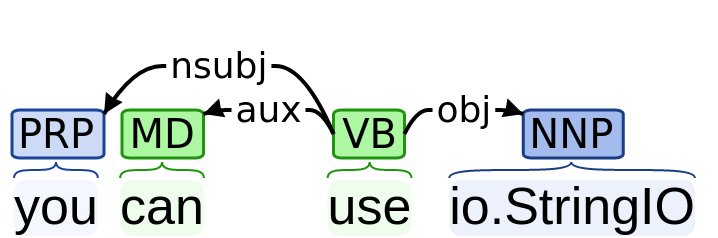
\includegraphics[width=0.40\textwidth]{cp2/textual-analysis.png}
%     \caption{Example of syntactic analysis}
%     \label{fig:syntactic-analysis}
% \end{figure}






% This section details empirical studies analyzing different aspects associated with 
%  natural language software artifacts.






% Early studies on textual analysis in software engineering often focused on program comprehension 
% and the text in the source code~\cite{Woodfield1981, maletic2002},
% but 
% Researchers have long recognized 
% that natural language artifacts 
% are rich in semantic information
% and that 
% better understanding these artifacts
% would lead to improved software~\cite{dekhtyar2004}.






% These studies have helped
% software engineering researchers make more informed decisions 
% on the design of automated tools 
% that identify and extract text from these artifacts---detailed further in this chapter. 




% The empirical analysis provided by these studies 
% has 
% deepened software engineering researchers' knowledge of the type of information available 
% in natural language artifacts 






% Bird at al. used it to investigate social aspects in development mailing lists~\cite{bird2006}. 
% They inspected nearly 102,000 messages on the Apache HTTP Server development lists
%  to find that character editing algorithms~\cite{levenshtein1966}, 
%  helped in unmasking developers' aliases, which helped investigating email 
%  exchange patterns of the key contributors of the project.


% .
% They have sampled 100 emails and identified that text for feature requests 
% often contain expressions in the form of suggestions
% (e.g., `\textit{we should add a new button}'), whereas solution proposals 
% are often expressed in the form of attempts (e.g., `\textit{let's try a new method to compute cost}')





% With regards to meta-data 




% \clearpage


% Several other studies have 
% investigated the meta-data available in
% natural language software artifacts. 
% % In Section~\ref{cp1:example},
% % we have presented an example of meta-data in a Stack Overflow post,
% %  other examples include fields in a bug report~\cite{Davies2014, Breu2010},
% % or tags and labels in GitHub projects~\cite{prana2019}.
% These studies often focus on 
% the frequency with which
% meta-data is available~\cite{Davies2014, bettenburg2008makes, uddin2015},
%  how up-to-date it is~\cite{ahmad2018, dig2006, shi2011}, 
%  and the perils of relying on meta-data for information extraction purposes.
% For example, Zhang et al. has shown that 
% certain comments on Stack Overflow are equally or more informative 
% that the information found in an accepted answer~\cite{zhang2019so}.


% has led software engineering researchers to 
% make more informed decisions on when to use meta-data 
% and how it can assist in the extraction of useful information from natural language 
% artifacts.
% For example, Wang et al. 


% found that 

% the number of votes 
% an answer has on Stack Overflow is 
% equally or more important than 


% ~\cite{wang2018}



% ~\cite{wang2018}









% Findings from these studies led 
% software engineering researchers to discuss the promises and perils of 
% using an artifact's meta-data~\cite{kalliamvakou2014, ahmad2018}.
% For example, an accepted answer on Stack Overflow 
% might not be the correct answer~\cite{wang2018}
% and 
% valuable information exists in elements not
% associated with any meta-data~\cite{zhang2019so},
% which we discussed as part of our 
% scenario about finding information about Android notifications (Section~\ref{cp1:example}).
% 


\section{Techniques for Mining Unstructured Text}
\label{cp2:general-approaches}




In this section, we provide background information on general 
approaches used
by software engineering researchers 
to identify text in natural language software artifacts~\cite{Bavota2016}.
We focus on 
automated approaches that might assist a person in discovering
text that addresses an information need,
presenting both core concepts needed to understand an approach 
and seminal work that has used an approach in 
the context of natural language software artifacts.



% For each approach, we detail 
% present seminal work that has applied 
% these approaches to problems related 
% to software engineering.
% These studies focus on specific tasks such as finding relevant passages in API documentation~\cite{Maalej2013,
% Petrosyan2015, Robillard2015}, learning about API types in code tutorials~\cite{Jiang2016b, Jiang2017},
% or detecting sentences that discuss a bug's expected behaviour~\cite{Chaparro2017}.
% These approaches respectively use the presence of code words, HTML anchor links, or whether a sentence contains
% a modal verb as properties to automatically identify relevant text.




\subsection{Pattern Matching}
\label{cp2:pattern-matching}



Pattern matching approaches use regular expressions describing
a sequence of tokens that represent
the text to be identified~\cite{Bavota2016}. 
We have shown how pattern matching identified
books whose subject contained
the keyword `\textit{android}' (Figure~\ref{fig:library-catalogue})
and the same principle could assist 
in finding parts of an artifact that contain some keyword, 
as many web browsers allow via a `\textit{find in page}' feature (Figure~\ref{fig:find-in-page}).
Nonetheless, this support is very limited and users would have to manually
inspect each match to 
determine if they are relevant or not.






\medskip
\begin{figure}[h!]
    \centering
    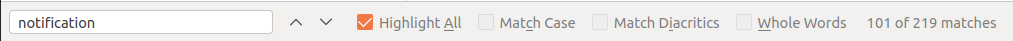
\includegraphics[width=\textwidth]{cp2/find.png}
    \caption{Find in page feature with results for the `\textit{notification}' term}
    \label{fig:find-in-page}
\end{figure}


More automated approaches have also been built using pattern matching, 
as when Panichella et al. 
matched class elements mentioned in development mailing 
 lists to source code files
to assist developers in finding information useful to 
 understanding the source code~\cite{panichella2012}.
Although the heuristics and regular expressions used in this and other studies (e.g.,~\cite{nadi2020, Maalej2013})
are lightweight and effective~\cite{Bavota2016}, 
pattern-matching approaches 
are often specific to certain kinds of domains and types of artifact~\cite{fucci2019}, 
limiting their use in the design of a generalizable technique.


% In development mailing lists, Panichella et al. 
% proposed an automatic approach leveraging \acf{IR} to extract 
% text with useful information that assists in understanding code elements inspected by a developer~\cite{panichella2012}




\subsection{Information Retrieval }
\label{cp2:information-retrieval}


\acf{IR} comprises techniques
or approaches for finding entities (documents, paragraphs, sentences, etc.)
that satisfy an information need~\cite{manning2010IR}.
At its most basic level, 
\acs{IR}
uses the 
frequency or co-occurrence of words (or phrases) to determine the relevance
of an artifact with regards to an information need, often expressed as an input query.


% For that, \acs{IR} identifies and structures all the words, or terms, 
% in an artifact so this information can be used for quick access. 
By counting how frequent  a word is in 
an artifact and across the entire collection of artifacts, 
\acs{IR} can be used to find which artifacts contain that word, or where within an artifact it appears. 
Using this principle, multiple \acs{IR} schemes have been proposed 
to identify text based on 
how not all the words in some vocabulary have the same weight (\textit{TF-IDF})~\cite{luhn1957tf, jones2004idf}, 
how to  represent sentences (\textit{VSM})~\cite{Salton1975vsm}, 
or how to account for different words that appear interchangeably in some context (\textit{LSI})~\cite{dumais1994latent}.



% Information retrieval applications span several disciplines and it has been used 
% to, for example, assist health workers in searching for medical records~\cite{hanauer2015}
% or to help law practitioners in understanding government regulations~\cite{lau2005legal}.

In natural language software artifacts, 
information retrieval has been used 
as part of approaches that
automatically identify sentences  that a developer would first read in a bug report 
when pressed with time~\cite{Lotufo2012},
or in approaches that help cluster software components to aid program comprehension of a software system~\cite{Marcus2003}.
In this dissertation, we combine information retrieval and word embeddings 
to identify relevant text across different kinds of artifacts, as Chapter~\ref{ch:identifying} further details.



\subsection{Natural Language Processing }
\label{cp2:nlp}


\acf{NLP} relies on the lexical or syntactical analysis of the text~\cite{jurafsky2014speech}
and such analyses might assist in the automatic identification of text that satisfies an information need. 
To illustrate some of the elements obtainable using \acs{NLP}, we consider a short sentence 
instructing how to perform a file system operation: ``\textit{you can use io.StringIO}''.
Figure~\ref{fig:nlp-analysis} shows elements extracted for this sentence using two \acs{NLP} techniques,
namely \acf{POS} tagging and dependency parsing.
The former assigns tags  ({\small \textit{PRP}, \textit{VP}, \textit{NNP},} etc.) to each word 
in a sentence~\cite{taylor2003penn} while the latter identifies
relationships between them, such as how 
`\textit{io.StringIO}' is the direct object (\textit{obj})
associated with the verb `\textit{use}'.



\medskip
\begin{figure}[h!]
    \centering
    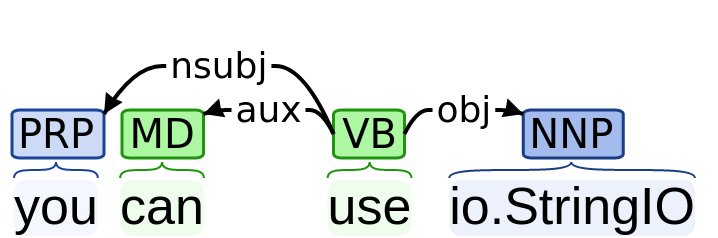
\includegraphics[width=0.40\textwidth]{cp2/textual-analysis.png}
    \caption{Syntactic elements for a sentence giving instructions about how to perform some file system operation}
    \label{fig:nlp-analysis}
\end{figure}


As an example of the application of \ac{NLP} to software engineering text,
Robillard  and Chhetri proposed a tool (Krec)
that uses \acs{POS} tagging to automatically 
identify text with threats and directives on how to use some API element~\cite{Robillard2015}.
As another example, {\small DeMIBuD}
is an automatic approach that uses dependency parsing
to automatically detect sentences discussing a bug's expected behaviour~\cite{Chaparro2017}.
In this work, we use \acs{NLP} as part of our 
analysis of the text deemed relevant to a set of software tasks (Chapter~\ref{ch:characterizing}).



\subsection{Machine Learning }
\label{cp2:machine-learning}



Several other studies have investigated the text 
of various kinds of natural language artifacts and 
the meta-data available on them~\cite{Ko2006, Maalej2013, Arya2019}.
Findings arising from these empirical studies
indicated regularities in the text and meta-data of 
an artifact which could be engineered into 
features that a  \acf{ML} technique could use to automatically identify or classify
text that addresses certain information need~\cite{Bavota2016}. 



Machine learning techniques can be categorized 
according to how they make use of available data. 
Supervised learning approaches use a set of features and labeled data
to train classifiers for detecting entities of interest (e.g., text, images, etc.)
while unsupervised learning approaches do not require labeled data and 
identify entities according to properties inferred from the data.



\subsubsection{Supervised Learning }
\label{cp2:supervised}


With regards to supervised learning approaches, 
we consider the families of classifiers that 
determine
\textit{(1)} if some entity belongs or not to a given class, as in binary classification
\textit{(2)} which class, out of many, some input entity belongs to, as in multinomial classification, or
\textit{(3)} which classes can be assigned to a given input, as in multi-label classification~\cite{alpaydin2020ml},
 and we detail their application to software engineering problems.



% Binary classifiers can be expressed as functions in the form of 
% $f(x) \arrowkeyright y$, where $x$ is a vector of features and $y \in {1, 0}$.
% Hence, it indicates whether $x$ belongs or not a given class.



Among other applications, binary classifiers have been used 
to classify text in bug reports that describes (or not) steps to reproduce a bug~\cite{Chaparro2016}
or  to classify paragraphs which contain explanations 
about API elements in a web tutorials\cite{Petrosyan2015}.
In turn, multinomial classifiers have been mostly used 
to identify a category, out of many, that represents the type of information 
associated with some text. For instance, Arya et al. identified 16 categories of  information available
in open source GitHub issues (e.g., workarounds, solution discussion, task progress, etc.)
and they proposed a multinomial classifier 
to automatically identify such categories~\cite{Arya2019}.
In a similar manner, Fu and colleagues consider 
five types of decisions that might arise during 
email exchanges (e.g., design, testing, management decisions, etc.)
and they proposed a multinomial classifier 
to automatically identify all the decisions present in emails of
a development mailing list~\cite{fu2021}.





Regardless of the type of classifier, these approaches are typically built 
with training data containing human-engineered features and the cost and effort of hiring skilled workers to produce 
the labeled data for these and other supervised learning approaches
has been a major limitation to their usage in software engineering research~\cite{Arpteg2018, ferreira2021}.




\subsubsection{Unsupervised Learning}
\label{cp2:unsupervised}



Common applications of unsupervised learning 
to natural language software artifacts 
comprise text summarization~\cite{Goldsteinet1999} and data clustering, which might help an individual both in understanding the key information in an 
artifact and also in deciding which information patches are 
 worth of their time~\cite{Lotufo2012}.


Unsupervised summarization approaches are often based on 
variations of the PageRank algorithm~\cite{Page1999}, and these approaches identify
the most central sentences in an artifact based on a set of relationships
established between all the sentences in that artifact.
Among other natural language artifacts,
extractive summarization techniques
have been applied to Stack Overflow posts~\cite{Ponzanelli2015},
coding tutorials~\cite{Li2018},
or bug reports, as
when Li et al. summarized 
key elements required to understand a bug and its resolution~\cite{li2018deep}.




A second family of unsupervised techniques focuses on clustering data.
These techniques use properties or features in the data to 
identify 
subsets with similar characteristics. 
Techniques that cluster data, such as \acf{LDA}~\cite{blei2003latent},
have been used by software engineering researchers to both 
bootstrap the categorization of information in 
natural language artifacts and as part of tools that identify topics in the text. 
For instance, Allamanis and Sutton
applied \acs{LDA}
to gain insight into the types of questions 
asked on Stack Overflow~\cite{Allamanis2013}
while FRAPT is a tool that 
uses \acs{LDA} to identity topics in a web tutorial
as well as relevant sentences in each of the topics identified~\cite{Jiang2017}.



Although unsupervised techniques lift the need for labeled training data,
they still use human-engineered features, 
which are often specific to certain 
types of artifact. Therefore, 
both supervised and unsupervised \acs{ML}
have limitations that might prevent their usage 
in the design of a generalizable technique.




\subsection{Deep Learning }
\label{cp2:deep-learning}



In contrast to the human-engineered features,
\acf{DL} approaches allow the automatic extraction of features 
from training data through a set of mathematical transformations~\cite{Deng2018, zhang2021deep}.
This makes 
deep learning an interesting 
approach to
uncover regularities 
that are not obvious or easily identified
by software engineering researchers.



A common application of \acs{DL} in software engineering is the usage of neural, or word, embeddings~\cite{Mikolov2013}
for information retrieval purposes. 
Neural, or word, embeddings produce vector representations in a continuous space,
where words with similar meanings are typically close in the vector space~\cite{harris1954distributional, mikolov2013efficient}. 
Researchers have found that word
embeddings mitigate lexical mismatches in the text found across different 
natural language software artifacts,
as shown by Ye et al.'s evaluation of word embeddings
for bug localization~\cite{Ye2016}
or Huang and colleagues' study on 
the usage of word embeddings for API recommendation~\cite{Huang2018}.
Guided by these findings, Chapter~\ref{ch:identifying} describes 
how we use word embeddings in the identification 
of task-relevant text.



Many other \acs{DL} studies in software engineering~\cite{ferreira2021,li2018deep}
use neural network architectures 
for the same range of problems discussed in Section~\ref{cp2:machine-learning}.
As explained by Watson et al.~\cite{watson2022},
neural network architectures are composed of several layers 
that perform a series of transformations on data passing through them. 
A set of parameters controls these transformations and 
adjust the model being trained so that it can predict 
the right outcome for any given input.
Using these concepts, researchers have proposed 
several  \acs{DL} architectures (e.g., \acs{RNN}s~\cite{rumelhart1986rnn, sutskever2014seq2seq}, encoder-decoders~\cite{bahdanau2014neural}, Transformers~\cite{Vaswani2017attention}, etc.) 
suitable for different problems. 
For instance,
Li et al. used an auto-encoder~\cite{liou2014autoencoder}
to produce more accurate and diverse summaries 
for bug reports~\cite{li2018deep} while 
Fucci et al. used a 
recurrent neural network (\acs{RNN}) 
to identify the types of information available in 
API documentation~\cite{fucci2019}.

% with \acf{LSTM}~\cite{hochreiter1997lstm}


Similar to supervised \acs{ML} approaches, deep learning approaches 
typically require large amounts of data for training purposes.
Nonetheless, recent advancements on the usage of
pre-trained models 
have lifted some of these limitations~\cite{erhan2010pre-train}.
In Chapter~\ref{ch:identifying},
we investigate how we can use a state-of-the-art architecture, namely BERT~\cite{Devlin2018Bert},
to identify relevant text across different types of artifacts.




% \subsection{Summary of Techniques}


% \art{Should I have a summary section and a table bundling examples of studies for each technique and the artifacts that they apply to? }






% Researchers pose the problem of identifying text 
% in a natural language artifact 
% as a binary classification problem. 
% That is, the use of a number of features 
% to predict whether the text is (or not)
% relevant to some context~\cite{aa}.
% In software engineering, 
% binary classifiers have been used for,
% for example, classify text that describes steps to reproduce a bug~\cite{Chaparro2016} or 
% classify text that explains a certain API element, as when 
% Petrosyan et al. used 
%  sentence-level features
% and meta-data features in a classifier 
% that 
% identifies explanations about an API element  in a web tutorial~\cite{Petrosyan2015}.




% Other classification problems predict which class, out of many, some input text belongs to. 
% This type of classification, referred to as multinomial or multi-class classification, 
% is of particular interest if 
% we consider the taxonomies described in Section~\ref{cp2:text-in-se}.
% For example, Arya et al. identified 16 categories of  information available
% in open source GitHub issues (e.g., workarounds, solution discussion, task progress, etc.)~\cite{Arya2019}
% and they proposed a multinomial classifier 
% to automatically identify such categories.








% Although valuable, these classifiers are instances of supervised learning methods.
% They require training data so that a classifier predicts the correct outcome 
% and the cost and effort of hiring skilled workers to produce 
% the labeled data for these and other supervised learning approaches
% has been a major limitation to their usage in software engineering research~\cite{Arpteg2018, ferreira2021}. As an alternative,
% researchers have also explored 
%  unsupervised learning methods---\acs{ML} techniques that do not required training data---for the automatic 
% identification or classification of the text in natural language artifacts~\cite{aa}.





% A common application of unsupervised learning in software engineering
% considers the automatic generation of text summaries.
% Most often, automatic summaries are produced 
% using extractive techniques that select a subset of 
% the sentences of an artifact that will compose the summary~\cite{a}.
% Among other natural language artifacts,
% extractive summarization techniques
% have been applied to Stack Overflow posts~\cite{a}, coding tutorials~\cite{a},
% or bug reports, as
% when Lotufo et al. 
% considered the kinds of sentences a developer would find relevant 
% to understand a bug report when pressed with time~\cite{Lotufo2012},
% and proposed an unsupervised summarization approach 
% based on the PageRank algorithm~\cite{Page1999}
% to identify these sentences. 




% A second set of unsupervised methods focus on clustering data.
% These techniques identify 
% subsets in the data that have similar properties or features 
% and techniques such as \acf{LDA}~\cite{blei2003latent}  have been used both to 
% bootstrap the categorization of information in 
% natural language artifacts and as part of tools that identify 
% portions of the text in an artifact that are helpful to some context. 
% As an example of the former, 
%  Allamanis and Sutton
% applied \acs{LDA}
% to gain insight into the types of questions 
% asked on Stack Overflow~\cite{Allamanis2013}.
% For the latter, tools such as FRAPT
% use \acs{LDA} to identity topics in a web tutorial
% and then extract sentences explaining API elements from each of the topics identified~\cite{Jiang2017}.


% Despite the significant contributions of these and other studies,
% one substantial challenge inherent to the supervised and 
% unsupervised \acs{ML} approaches 
% is that researchers must engineer which 
% features their \acs{ML} technique will use~\cite{ferreira2021}.
% Hence, \acs{ML} approaches have limitations similar to the pattern 
% matching approaches when we consider 
% the specificity and cost of engineering such features
% for a variety of kinds of artifacts.








% pre-trained models that do not require large amounts of training data to our domain problem~\cite{devlin2018bert, Ye2016}. With this approach, we revisit findings on the trade-offs of using machine learning techniques to mine textual data~\cite{Chaparro2017, Bavota2016}.




% using them as a way to compare the semantic similarity of the text~\cite{mihalcea2006}.
% Guided by the recent success of word embeddings 
% for a variety of software development 
% activities,,
% Chapter~\ref{ch:identifying} 
% describes how we incorporate word embeddings in the 
% design of techniques that automate the identification of task-relevant text. 






% ,
% thus allowing \acs{DL}
% to automate the identification of text in natural language software artifacts
% with these `hidden' properties. 









% These studies focus on specific tasks such as finding relevant passages in API documentation~\cite{Maalej2013,
% Petrosyan2015, Robillard2015}, learning about API types in code tutorials~\cite{Jiang2016b, Jiang2017},
% or detecting sentences that discuss a bug's expected behaviour~\cite{Chaparro2017}.
% These approaches respectively use the presence of code words, HTML anchor links, or whether a sentence contains
% a modal verb as properties to automatically identify relevant text.
% Given how quickly developers progress to using new kinds of technology to
% record pertinent information (e.g., slack~\cite{Storey2017, Lin2016}),
% it may be difficult to scale such artifact-centric approaches to cover the range of
% artifacts that could be returned from a search.
% A second issue arises from the fact that coding procedures used to determine relevancy
% in these studies do not consider disagreements~\cite{Stol2015}.
% That is, there are many criteria in how individuals
% assess relevance~\cite{Barry1994, Barry1998, Freund2015}
% and there are no guarantees that
% developers will use the same properties to determine text relevant to their tasks~\cite{Freund2013, Freund2015}.
% In contrast, our study does not pre-assume any relevance cues, and instead,
% we leave the decision of what text is perceived as relevant to a particular task to
% the participants in our experiment.









% Knowledge Recommender ()
% is an example of a
%  tool that uses lexical patterns to 
%  automatically detect relevant text in  API documentation. 
% Krec's premise is that relevant sentences contain a code element, such as a method or class signature.
% These code elements are identifiable via regular expressions 
% and Krec contains a catalog of 361 unique patterns 
% that identify threats and directives on how to use some API element.
% For example, Krec uses the pattern {\small \textit{$\{$may}, \textit{efficient}, \textit{code element regex$\}$}} 
% to identify sentences giving instructions about an efficient way to 
% perform some operation. 



%  is a linguistic-based approach that 

% It uses a set of 154 discourse patterns
% derived from nearly 3,000 bug reports 
% to identify such sentences. 
% For example, the pattern 
% {\small \textit{$\{$subject}, \textit{should/shall (not)}, \textit{complement$\}$}}
% captures common ways with which developers describe a system's expected behaviour
% and empirical assessment of the patterns used by the tool has shown that it 
% detects sentences of interest in bug reports with high accuracy.



% ~\cite{krallinger2017}



% ~\cite{mcdonough2019}
% 



\section{Task-specific Techniques}
\label{cp2:task-approaches}



Although certainly valuable, the techniques mentioned in Section~\ref{cp2:general-approaches}
do not extract text tailored to 
a specific software task. In other words, they identify 
a set of sentences in an input artifact regardless of the developer's task. 
In contrast, this section focuses on task-specific techniques.
% where core component to identifying information specific to a task 
% is a query which represents the task being performed~\cite{Bavota2016}. 
% This query can be explicitly formulated by a developer 
% or implicitly derived from the code or the context 
% in which a developer is working.

%  (as described in Section~\ref{cp2:unsupervised})
A small number of studies~\cite{Xu2017, silva2019, liu2019qapi} 
 formulate the problem of identifying task-specific text 
 in specific types of artifacts as 
a special case of query-based summarization~\cite{Goldsteinet1999}. That is, 
instead of producing a summary for the entire content of 
an artifact,
these studies first use information retrieval techniques
to identify a subset 
of sentences relevant to a task and then, 
a summary of these key sentences is produced.



AnswerBot~\cite{Xu2017} is an example of a query-based summarization tool.
It uses word embeddings to find which sentences in a Stack Overflow answer 
are most similar to a query representing a developer's task.
The tool uses semantic similarity in conjunction with 
Stack Overflow's meta-data to decide which text  it should include
in the summary that it will produce. 
A second query-based summarization tool by Liu et al. parses the content 
of API documents to build a knowledge graph of the information within this type of artifact. 
Their tool, KG-APISumm~\cite{liu2019qapi}, uses this graph 
to find nodes with text that matches the text of an input task, 
producing a task-specific summary for this type of artifact. 


These techniques
target one type of artifact and they also use an artifact's meta-data to 
assist in the automatic identification of task-relevant text, thus
limiting their use across the
many different kinds of artifacts developers encounter
daily in their work. 
For example, AnswerBot uses the number of votes an answer has to decide which text it will use to produce a summary~\cite{Xu2017}
while KG-APISumm uses 
code blocks, HTML anchor links and other properties exclusive to API documents to build the knowledge graph used as part of its summarization approach~\cite{liu2019qapi}.
We differ from these studies 
by not using assumptions 
specific to certain kinds of artifacts
and by considering how to identify task-relevant text 
in a more generalizable manner.





% As a result, these approaches are constrained to specific artifacts and do not 
% generalize to the different kinds of artifacts a developer might consult. 





% the text identified by these techniques might indeed 


% contain information relevant to a specific software task,
% a key component that distinguish the techniques 
%  is that they 




% We now consider applications that assist developers in 
% searching for artifacts that contain information 
% for a particular task
% and that automate the identification 
% of text likely relevant to a developer's task;




% We use the terms change task and task to refer to any change to a software system that serves a predefined purpose, such as a bug fix or an enhancement.


% In this section, we detail textual approaches that automate the identification 
% of text likely relevant to a developer's task. 



% Task-specific automated approaches 
% use many of the techniques discussed in Section~\ref{cp2:general-approaches}
% in conjunction with the text in a developer's task
%  or the code in a developer's workspace
% as potential ways  
% to identify task specific information.
% A seminal tool that exemplifies 
% how these sources assist in locating task specific information is
% Hipikat~\cite{Cubranic2005}.
% It takes a query explicitly prompted by a developer 
% or implicitly based on the code that the developer 
% has inspect and  
% it recommends artifacts from a project's archive 
% that are pertinent to the query.
% While Hipikat makes recommendations at the artifact level,  
% this approach could be fine-tuned to identify 
% parts of an artifact that are relevant~\cite{Cubranic2005}
% and other studies have since built upon this core idea. 
% For example, Deep Intellisense 
% uses pattern matching to 
% identify 
% artifacts containing text that 
% would assist a developer
% better understand the code that they inspect~\cite{Holmes2008}
% while 
% CueMeIn takes the code 
% a developer is currently editing and it
% automatically finds 
% excerpts from web tutorials 
% that might contain explanations 
% for the classes and methods 
% of the method being edited~\cite{sun2021}. 










% In Section~\ref{cp2:general-approaches}, we described 
% techniques for mining textual data. 
% These techniques identify text that might assist a developer 
% in performing certain activities such as finding 
% text describing how to use an API~\cite{Robillard2015} 
% or finding text with decisions made by members of a development 
% community~\cite{fu2021}.
% 



\section{Improving Developers' Productivity}
\label{cp2:dev-productivity}


\art{stopped reviewing related-work here}


% The tools and approaches presented in Sections~\ref{cp2:general-approaches}
% and~\ref{cp2:task-approaches}
% are examples of studies that help developers in locating 
% information that assists them in completing a software task.
% These studies fit in the bigger context 
% of software engineering research 
% facilitating or improving the quality of a developer's work~\cite{Kersten2006, Meyer2017, satterfield2020}. 





% As part of their work, developers engage in many sensemaking and decision-making activities~\cite{sillito2006} and several studies have investigated how to 
% provide means to better  
% assist developers in performing such activities~\cite{Liu2018Unakite, liu2021, barnett2015}.
% For example, 
% Ponzanelli et al. proposed a tool, Libra, that monitors the web pages a developer 
% has navigated and uses that to show 
% how similar or not the results of a new web search are in comparison to the already navigated 
% pages, which offers contextual information-seeking support~\cite{Ponzanelli2017}.



% Researchers have also been interested in 
% making knowledge bases
% that developers working on a task can benefit from. 
% In Section~\ref{cp2:task-approaches} 
% we cited Hipikat~\cite{Cubranic2005}, a seminal tool that exemplifies this concept in action.
% Based on the current code being inspected by a developer or based on a query prompted by a developer, 
% it recommends artifacts from a project's archive 
% that are pertinent to the code being inspected.
% This archive, or project memory, is produced 
% based either on relationships between the artifacts in a software project 
% or based on the source code changed in a bug fix or feature request~\cite{Cubranic2005}.
% Other tools like Strata summarize knowledge produced by developers 
% while they navigate on the web so that other developers
% can use this knowledge to have a 
%  head start when performing similar tasks~\cite{liu2021}.




% We build upon many of the research procedures outlined 
% in these and many other studies in the field. 
% For example, in the evaluation of Strata, 
%  Liu et al. describe procedures 
% considering how a control and tool-assisted group 
% complete information-seeking tasks~\cite{liu2021},
% which assisted in the design of our experiment for 
% evaluating an automated approach to
% task-relevant text identification (Chapter~\ref{ch:assisting}).







